\let\negmedspace\undefined
\let\negthickspace\undefined
\documentclass[article]{IEEEtran}
\usepackage[a5paper, margin=10mm, onecolumn]{geometry}
%\usepackage{lmodern} % Ensure lmodern is loaded for pdflatex
\usepackage{tfrupee} % Include tfrupee package

\setlength{\headheight}{1cm} % Set the height of the header box
\setlength{\headsep}{0mm}     % Set the distance between the header box and the top of the text

\usepackage{gvv-book}
\usepackage{gvv}
\usepackage{cite}
\usepackage{amsmath,amssymb,amsfonts,amsthm}
\usepackage{algorithmic}
\usepackage{graphicx}
\usepackage{textcomp}
\usepackage{xcolor}
\usepackage{txfonts}
\usepackage{listings}
\usepackage{enumitem}
\usepackage{mathtools}
\usepackage{gensymb}
\usepackage{comment}
\usepackage[breaklinks=true]{hyperref}
\usepackage{tkz-euclide} 
\usepackage{listings}                                       
\def\inputGnumericTable{}                                 
\usepackage[latin1]{inputenc}                                
\usepackage{color}                                            
\usepackage{array}                                            
\usepackage{longtable}                                       
\usepackage{calc}                                             
\usepackage{multirow}                                         
\usepackage{hhline}                                           
\usepackage{ifthen}                                           
\usepackage{lscape}

\renewcommand{\thefigure}{\theenumi}
\renewcommand{\thetable}{\theenumi}
\setlength{\intextsep}{10pt} % Space between text and floats

\numberwithin{figure}{enumi}
\renewcommand{\thetable}{\theenumi}

% Marks the beginning of the document
\begin{document}
\bibliographystyle{IEEEtran}
\title{NCERT-8.2.3}
\author{EE24BTECH11035 - KOTHAPALLI AKHIL}
{\let\newpage\relax\maketitle}

\noindent\textbf{Question: }  
Find the area of the region bounded by the curves $y = x^2 + 2$, $y = x$, $x = 0$, and $x = 3$.\\
\solution \\
\textbf{Theoritical approach: }\\
The area of the region can be expressed as:
\begin{align}
   A = \int_0^3 \left( x - (x^2 + 2) \right) dx. 
\end{align}

Simplify the integrand:
\begin{align}
A = \int_0^3 \left( -x^2 + x - 2 \right) dx.
\end{align}
on integration,
\begin{align}
    A={\left[-\frac{x^3}{3}+\frac{x^2}{2}-2x\right]_0}^3
\end{align}
on applying the limits,
\begin{align}
   A=(-\frac{3^3}{3}+\frac{2^2}{2}-)6-(0+0-0)
\end{align}
\begin{align}
    A=-10.50
\end{align}
Here, we are getting A negative .That means it is area under the X-axis.
Therefore,the maginitude of theoritical area is 10.50.\\
\textbf{Using the trapezoidal method,}\\ Divide the interval $[0, 3]$ into $n$ subintervals of width $h = \frac{3-0}{n} = \frac{3}{n}$. Let $x_0 = 0$, $x_1 = h$, $x_2 = 2h$, $\dots$, $x_n = 3$.

The trapezoidal method for numerical integration is given by:
\begin{align}
  A \approx \frac{h}{2} \left[ f(x_0) + 2\sum_{i=1}^{n-1} f(x_i) + f(x_n) \right]  
\end{align}

where $f(x) = -x^2 + x - 2$.

Substitute $f(x)$ into the formula:
\begin{align}
    A \approx \frac{h}{2} \left[ (-x_0^2 + x_0 - 2) + 2\sum_{i=1}^{n-1} (-x_i^2 + x_i - 2) + (-x_n^2 + x_n - 2) \right].
\end{align}


Thus, the for the area can be written as:

\begin{align}
  A = \frac{h}{2} \left[ f(x_0) + 2\sum_{i=1}^{n-1} f(x_i) + f(x_n) \right].  
\end{align}


\textbf{Numerical Approach}\\

To approximate the area of the region using the trapezoidal method, we adopt the following numerical approach. This method involves iteratively calculating the area using discrete steps:

\textbf{Initialization:}
\begin{itemize}
    \item Start with initial values $x_0 = 0$ and $A_0 = 0$.
    \item Set the step size $h = \frac{3}{n}$, where $n$ is the number of subintervals.
\end{itemize}

\textbf{Difference Equation:}\\
\begin{itemize}
    \item For each iteration $i$ from 1 to $n$, perform the following steps:
    \begin{itemize}
        \item[1.] Compute $y_i = -x_i^2 + x_i - 2$.
        \item[2.] Update the area sum using:
        \begin{align}
        A_{i} &= A_{i-1} + \frac{1}{2} h (y_{i} + y_{i-1})
        \end{align}
        \item[3.] Update $x_i$ for the next iteration using:
        \begin{align}
        x_{i} &= x_{i-1} + h
        \end{align}
    \end{itemize}
\end{itemize}

\textbf{Final Area Calculation:}\\
\begin{itemize}
    \item After completing all iterations, the final approximate area $A_n$ is:
    \begin{align}
    A &= A_n
    \end{align}
\end{itemize}

\textbf{Initial Conditions:}
\begin{itemize}
    \item $x_0 = 0$
    \item $A_0 = 0$
    \item $h = \frac{3}{n}$ (depending on the chosen number of subintervals $n$)
    \item Here we assume $n = 500$.
\end{itemize}

This approach ensures an accurate approximation of the area by iteratively applying the trapezoidal rule, leveraging the discretized nature of the integral.\\
$ \implies$ The theoritical value of Area is 10.50\\
 $ \implies$ The computational value of Area is 10.505.\\
 Therefore, we can claim that trapezoidal rule/method for finding area works well.
 \begin{figure}[h!]
	\centering
	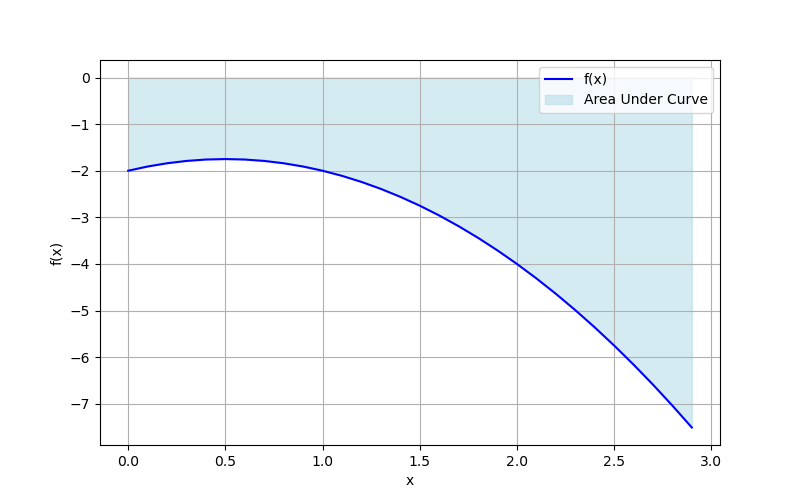
\includegraphics[width=\columnwidth]{figures/Figure_1.png}
	\caption{Area function graph.}
	\label{stemplot}
\end{figure}
\end{document}



